\documentclass[a4paper]{article}

\usepackage[T1]{fontenc}
%\usepackage[utf8]{inputenc}
\usepackage[italian]{babel}
\usepackage{amssymb}
\usepackage{hyperref}
\usepackage{mathtools}
\usepackage{amsthm}
\usepackage[ruled,vlined,noend]{algorithm2e}

%%%%%%%%%%%%%%%%%%%%%%%%%%%%%%%%%%%%
\usepackage{listings} 
\lstdefinestyle{mystyle}{
    breakatwhitespace=false,                   
    captionpos=b,                    
    keepspaces=true,                 
    numbers=left,                    
    numbersep=5pt,                  
    showspaces=false,                
    showstringspaces=false,
    showtabs=False,                  
    tabsize=2
}

\lstset{style=mystyle}

\usepackage{setspace}
\singlespacing
%%%%%%%%%%%%%%%%%%%%%%%%%%%%%%%%%%%%
\usepackage{ulem} 
\usepackage{soul}

\usepackage{graphicx}
\graphicspath{ {./images/} }
%%%%%%%%%%%%%%%%%%%%%%%%%%%%%%%%%%%%

\mathtoolsset{showonlyrefs}  
\hypersetup{
    colorlinks=true,
    linkcolor=black,
    filecolor=black,      
    urlcolor=black,
}

\newcommand{\pluseq}{\mathrel{{+}{=}}}

\newtheorem{theorem}{Theorem}
\newtheorem{corollary}{Corollary}
\newtheorem{lemma}{Lemma}
\newtheorem{remark}{Remark}
\newtheorem{definition}{Definition}

\setcounter{secnumdepth}{3}
\setcounter{tocdepth}{3}

\title{Architectures for Big Data - First assignement}
\author{Federico Cristiano Bruzzone \& Andrea Longoni}
\date{}
%\makeindex

\begin{document}
\maketitle
\newpage
% \setlength{\parskip}{0.15em}
% \tableofcontents
\setlength{\parindent}{0pt}
\setlength{\parskip}{0.8em}
\newpage

%\section{section}
...

\subsection{subsection}
	
\paragraph{paragraph}

\begin{remark}
    ...
\end{remark}

\subsubsection{subsubsection}

\subsubsection{subsubsection}

\paragraph{paragraph}

\subsection{subsection}
...
\begin{enumerate}
    \item 
    \item
    \item 
\end{enumerate}

\begin{itemize}
	\item 
    \item 
\end{itemize}

\begin{theorem}
    $PO \subseteq NPO$
\end{theorem}
\begin{proof}
    ...
\end{proof}

\begin{equation}
    \begin{aligned}
        \mathit{APX} = \{\Pi | \Pi \mathit{\;di\;ottimizzazione\;t.c.\;}
\exists \rho \geq 1, A, \\\mathit{t.c\;} x\rightarrow A \rightarrow y(x)\;\mathit{con}\;R_\Pi(x, y) \leq \rho\}
    \end{aligned}
\end{equation}


\paragraph{Algoritmo di risoluzione}
L'algoritmo di risoluzione è abbastanza semplice e si basa sulla 
ricerca di un cammino aumentante.

\begin{algorithm}[H]
    \SetAlgoLined
    \KwIn{$G=(V,E)$}
    \KwResult{Matching $M$ per $G$}
     $M \gets \emptyset$\\
     \While{$\Pi = \mathit{findAugmenting(G)}$}{
        $M.update(\Pi)$
     }
     \Return{M}
     \caption{BiMaxMatching}
\end{algorithm}


\subsection{Tecniche greedy}
Nella sezione a seguire si presentano problemi di ottimizzazione per cui 
tecniche greedy funzionano abbastanza bene. 
I problemi affrontati sono quelli di \emph{Load Balancing}, \emph{Center Selection} e \emph{Set Cover}.

\subsubsection{Load balancing}
\label{lb}
Il problema di Load Balancing può essere visto come il compito
di assegnare a macchine dei lavori da compiere, che richiedono del tempo, 
in modo da minimizzare il tempo totale.


\begin{theorem}
    Load Balancing è NPO completo
\end{theorem}
Bisogna perciò trovare un modo di approssimare una soluzione.
\paragraph{Greedy balance}
Il primo approccio alla risoluzione del problema è quello di assegnare la prossima
task alla macchina più scarica in questo momento.

\begin{algorithm}[H]
    \SetAlgoLined
    \KwIn{$M$ numero di macchine, $t_0, \dots, t_n$ task}
    \KwResult{Assegnamento delle task alle macchine}
     $L_i \gets 0\;\forall i \in M$\\
     $\alpha \gets \emptyset$\\
     \For{$j = 0, \dots, n$}{
         $\hat{i} = \min(L_i)$\\
         $\alpha(j) = \hat{i}$\\
         $L_{\hat{i}} \pluseq t_j$
     }
     \Return{$\alpha$}
     \caption{GreedyBalance}
\end{algorithm}

\begin{lstlisting} %[language=Python, caption=Python example]

import numpy as np
    
def incmatrix(genl1,genl2):
    m = len(genl1)
    n = len(genl2)
    M = None #to become the incidence matrix
    VT = np.zeros((n*m,1), int)  #dummy variable
    
    #compute the bitwise xor matrix
    M1 = bitxormatrix(genl1)
    M2 = np.triu(bitxormatrix(genl2),1) 

    for i in range(m-1):
        for j in range(i+1, m):
            [r,c] = np.where(M2 == M1[i,j])
            for k in range(len(r)):
                VT[(i)*n + r[k]] = 1;
                VT[(i)*n + c[k]] = 1;
                VT[(j)*n + r[k]] = 1;
                VT[(j)*n + c[k]] = 1;
                
                if M is None:
                    M = np.copy(VT)
                else:
                    M = np.concatenate((M, VT), 1)
                
                VT = np.zeros((n*m,1), int)
    
    return M
\end{lstlisting}

%%%%%%%%%%%%%%%%%
\usepackage{listings}
\usepackage{xcolor}

\definecolor{codegreen}{rgb}{0,0.6,0}
\definecolor{codegray}{rgb}{0.5,0.5,0.5}
\definecolor{codepurple}{rgb}{0.58,0,0.82}
\definecolor{backcolour}{rgb}{0.95,0.95,0.92}

\lstdefinestyle{mystyle}{
    backgroundcolor=\color{backcolour},   
    commentstyle=\color{codegreen},
    keywordstyle=\color{magenta},
    numberstyle=\tiny\color{codegray},
    stringstyle=\color{codepurple},
    basicstyle=\ttfamily\footnotesize,
    breakatwhitespace=false,         
    breaklines=true,                 
    captionpos=b,                    
    keepspaces=true,                 
    numbers=left,                    
    numbersep=5pt,                  
    showspaces=false,                
    showstringspaces=false,
    showtabs=false,                  
    tabsize=2
}

\lstset{style=mystyle}
\section{Overview}

The assignment is focused on implementing a simple Architecture using Python Abstract Classes to build a structure that is lead to retrieve data from generics externals data source for importing them into an internal DB that will be used from the analyst’s team for analysis purposes.

\section{Project Requirements}

The project requirements are reduced to the ideation and abstract implementation of a software architecture which satisfies to follow the \textit{Software Architecture Pillars} seen during the class lessons.

In specific those pillars are:

\begin{enumerate}
	\item Being the framework for satisfying requirements
	\item Being the technical basis for design
	\item Being the managerial basis for cost estimation and process management
	\item Enabling component reuse
	\item Allowing a tidy scalability 
	\item Avoiding handover and people lock in
\end{enumerate}

\section{Software Architecture Pillars}

\subsection{Being the framework for satisfying requirements}

\begin{center}
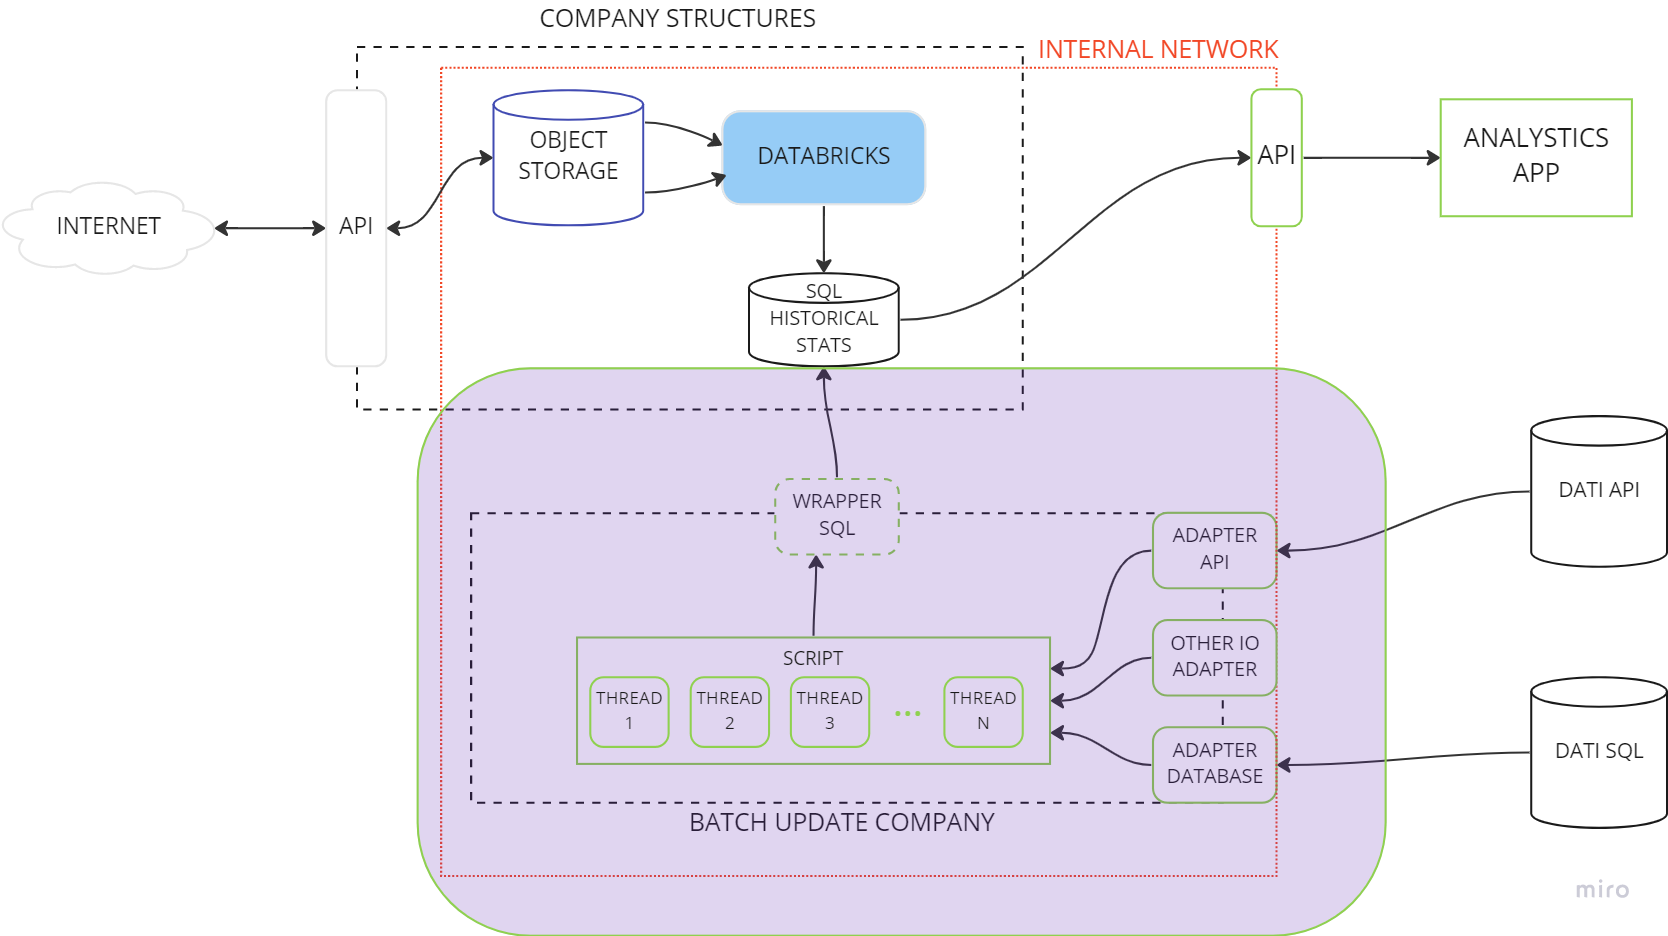
\includegraphics[scale=0.4]{scheme-diagram}
\end{center}

\subsubsection{Functional Requirements}

The software will need the ability to read data from generic external sources (like Databases, public API, Data Stream, …) and to prepare and process them before their insertion inside the local Company Historical DB.

This software, that furthermore we will call ‘Batch Extractor’, will need to be able to adapt itself for retrieving data from any data source that the company will identify as important to be importable inside the system for allowing analysts to be free of finding whatever data source should fit better for their needs.

The batch system will also need to be adaptable for changes on the internal structure of the Company, in particular the DB, for letting free the company to make the best business and behavioral choices in any moment free of the current implementations of the system.

Important will also be that the structure should be scalable on multiple and concurrent input data source, for allowing the system to inject data at different speeds based on the need of the analyst and the environment.

\subsubsection{Technical Requirements}

Due to accomplish the necessity of the structure of being adaptable to any external source, is important that the software will presents a layer of external adapters that will be used to connect to the external sources for retrieving properly data based on the external infrastructures and needs. 

Important will also be the possibility for the system to be able to add new adapters to interact with new outside data sources. Those will simply need to pass the data to the script unknowingly of the internal DB implementation and this will then take care of them for the inserting inside the Historical DB.

Important will also be the presence of wrappers for the connection with the internal Historical DB. 
This feature will provide another abstraction layer that will be important to allow the company to apport in any moment whatever changes on the internal technologies used for storing data.

\subsubsection{Security Requirements}

The system will need to be placed inside the company network due to avoid the necessity of opening external ports directly to the Historical DB, for reduce the possibility of penetration of malicious actors inside the system.

Important will also be the process of input sanitization after receiving data from the external source and before inserting them inside the queries, due to avoid the exposure of the system to attack like SQL injection or similar.

\subsection{Being the framework for satisfying requirements}

The development of the architecture, later illustrated, has been done keeping in mind that we will have a single immutable database (historical database) on which we will write and possible multiple databases or data sources from which we will read.

To interface on these databases (or data sources) we thought to use multiple adapters to transform the inbound data in a writable format for the Historical DB.

\begin{center}
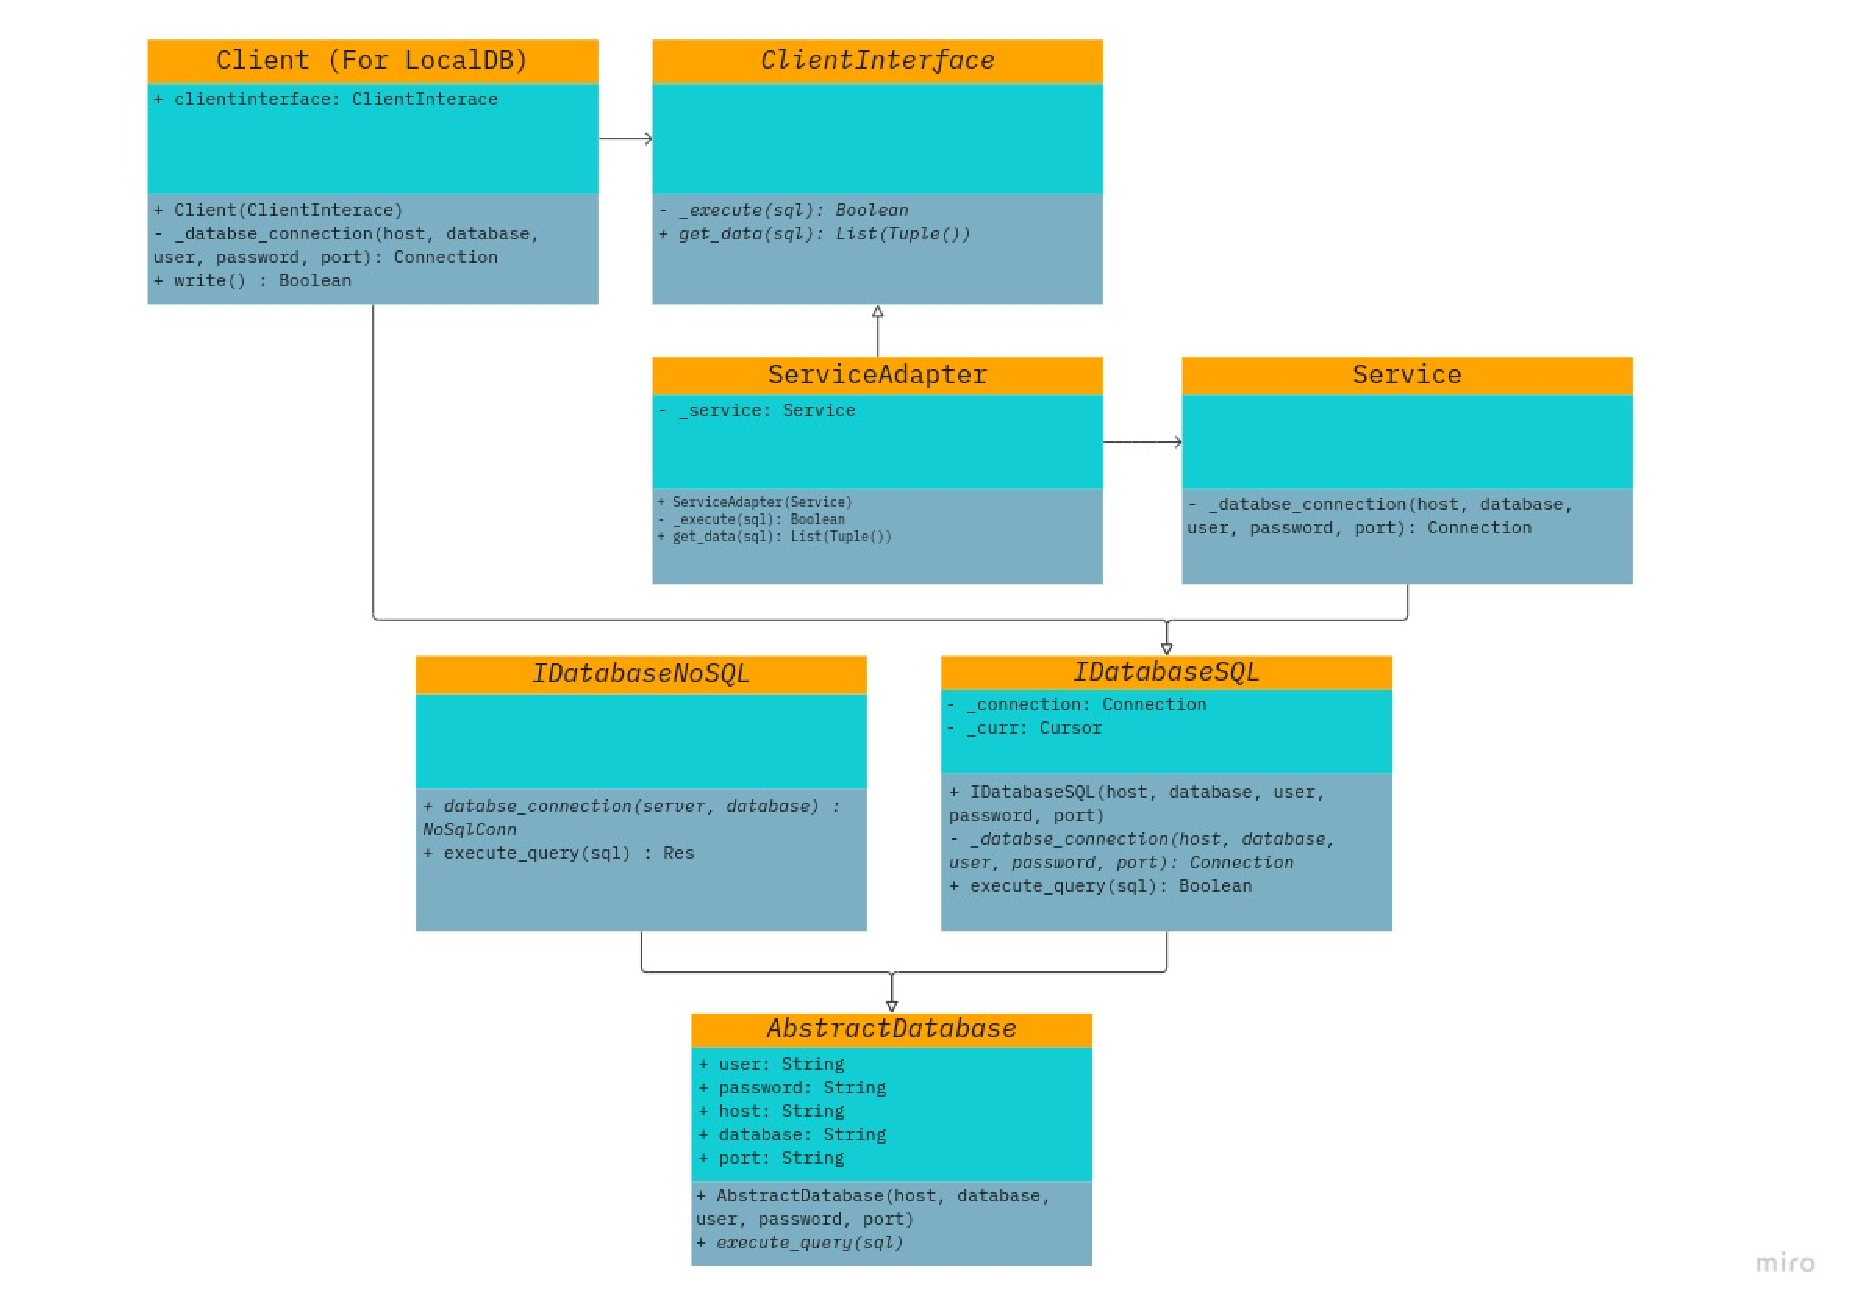
\includegraphics[scale=0.45]{uml-diagram}
\end{center}

\textbf{Please note: The gray part is not implemented. We will talk about it in the reusability chapter.}

We have thought to use Adapter (Wrapper) pattern, because this will allow us to keep the same historical database and make it be able to communicate with the different types of external data source.

This implementation uses the object composition principle: the adapter implements the interface of one object and wraps the other one.

\begin{enumerate}
	\item \textit{AbstractDatabase} is an abstract class that contains the information for connecting with any database.
     
     In the inherited class, you will have to implement execute\_query(...) method.

	\item \textit{IDatabaseSQL} is an abstract class that define behavior of the SQL database.
     
     Since IDatabaseSQL inherits from AbstractDatabase it must implements execute\_query(...) method.
     
     In the inherit class, you will have to implement \_database\_connection(...) method.

     Assuming that in python any database sql library implement .connector.connect(...) and .cursor() methods: 
\begin{enumerate}
	\item we use \_connection field to store the connection to the specific database;
	\item we use \_cursor field to store the cursor to the specific database.
\end{enumerate}

Note that \_cursor contanis the .execute(...) method that is used to execute the query.

	\item \textit{ExternalDatabase} is a concrete class that allow us to establish a connection.
	
     Since ExternalDatabase inherits from IDatabaseSQL it must implements \_database\_connection(...).

	\item \textit{ExternalDatabaseAdapter} is a concrete class that allow data from ExternalDatadase to be readable and writable for HistoricalDatabase. 
	
     Since ExternalDatabaseAdapter inherits from IHistoricalDatabse it must implements \_read\_from(...) and \_execute(...) methods.
     
     Since ExternalDatabaseAdapter has an ExternalDatabase object instance inside, it will have the ability to execute query from it and therefore having the ability to read data from it.

	\item \textit{IHistoricalDatabse} is an interface that contains the delcarations of methods that must be implemented by each adapters.
	
     We expect the read\_from(...) mothod to return a fitted content for the HistoricalDatabase. 

	\item \textit{HistoricalDatabse} is a concrete class that contains methods to execute query into the historical database.
	
     Since HistoricalDatabse inherits from IDatabaseSQL it must implements \_database\_connection(...).
    
     Since HistoricalDatabse has a IHistoricalDatabase object it can get data from it.
     
     To remember the last item we have read, we store its identifier (ordered) into a sync.json file, and when we will have to execute the next query, we'll read from sync.json the identifier.
        
     The .write\_to(...) mothod use the .read\_from(...) method of the adapter to get a list of tuple and then insert them into the historical database. 
     
     After this, it will commit the changes.
\end{enumerate}

\subsection{Being the managerial basis for cost estimation and process management}

\begin{lstlisting}[language=Python, numbers=none]
Infrastructure Cost: Physical Server owning:    4 x 9000$ = 36000$
                     Estimated power:           4 x 250$ = 1000$/month
                     Estimated internet access: 2250$/month
     Developer Cost: 3 Agents:                  30000$
                     Software developing:       35000$
                     Network adapt:             20000$
 Algorithmical Cost: Business logics:           10000$
   Maintenance Cost:                            20000$/Year


        TOTAL COSTS: One Shot:                  131000$
                     Running:                   57K000/Year 
\end{lstlisting}

\textbf{Infrastructure Specs}

Physical Server: 4 * ProLiant DL385 Gen10 Plus : 9,000.00 

Power costs:     4* 1600W (Server alimentation) = 6400W * 13c\$/KwH : 1000\$

Internet costs:  Dedicated Internet Access, 40Gbps IP Transit: 2250\$/month

Developer cost:  Based on 6 months working\\

\subsection{Enabling component reuse}

\begin{lstlisting}[language=Python]
class IHistoricalDatabse(ABC):
    @abstractmethod
    def _execute(self, sql): pass

    @abstractmethod
    def read_from(self, sql): pass

class ExternalDatabaseAdapter(IHistoricalDatabse):
    external_databse: ExternalDatabase = ''

    def __init__(self, external_databse: ExternalDatabase):
        self.external_databse = external_databse
        print('ExternalDatabaseAdapter has been created')

    def _execute(self, sql):
        query_res = self.external_databse.execute_query(sql)
        return query_res
    
    def read_from(self, sql):
        query_res = self._execute(sql) 
        return query_res   
\end{lstlisting}

Talking about reusability, as you can see in the uml diagram in chapter 1.2, the not implemented gray parts are just examples of external sources that could be implemented if we will need to read from other services. 

Doing so we we'll not have to change each time the way we are going to write into the internal DB, because the adapter will achieve the goal to manage the importing of data inside the script. From here then the data will be passed by the wrapper to the internal DB.

Obviously, it you want to create a new adapter, you will have to code a class which will inherit from IHistoricalDatabase. This allow the historical database, which contains an IHistorical database object, to not change the internal code.

\subsection{Allowing a tidy scalability}

The system has been ideated and structured to be scalable on the quantity of data received in input from the external sources.
This choice born from the unknown of the availability of data during time on the remote source.

Allowing this scalability help the system to be ready for situations where the data are given “real time” and are not retrievable in a second moment. For not losing data will be important for the system to be able to adapt his capability of reading data without losing on performance or reliability.

At this purpose the script will have more internal threads that will be capable of increasing in number when there will be high inbound traffic and then reduce themselves when not anymore necessary.

\subsection{Avoiding handover and people lock-in}

The problem of vendor lock-in is commonly forcing the company to be stuckked to use some internal technologies that cannot be changed because the cost of the replacement would be higher than the benefits. This problem can also raise on company’s employees when the develop of code has not been well documented and the company find herself to be in the position to cannot replace an employee due to his only known about the project code.

To avoid those problem the solution proposal has been to implement an internal wrapper between the script and the internal DB to allow in a second moment to be able to change internal technologies configurations and from the employees prospective we provide a fully code documentation to let any new future worker on the project be able to understand every snip of code what is doing and how to manage them in case of bug or unexpected behavior.

\section{Testing}

We have tested the code by creating table \textbf{user1} and \textbf{user2} with \textit{id} (Primary Key, Auto Increment), \textit{name} and \textit{surname} respectively and then we have tried to read from \textbf{user1} and write to \textbf{user2}.

We have used sync.json file to store the last tuple that we have read from the \textbf{user1}.

Reading this file we were able to resume reading \textbf{user1} from the last writing in table \textbf{user2}, whitout reading the whole database every time.

For simplicity, we have been using the id of the \textbf{user1} table to keep track of the last tuple stored in the sync.json file, and we have read and wrote in the same database instance.

Our tests were performed succesfully.


\textbf{First execution}
\begin{lstlisting}
Connection successfull to the: 
          127.0.0.1 test_database root welcome123 
ExternalDatabaseAdapter has been created
Connection successfull to the: 
          127.0.0.1 test_database root welcome123 

Query has been executed: 
          SELECT name, surname FROM user where id > 0
          ('federico', 'bruzzone')
          ('andrea', 'longoni')
          ('massimiliano', 'visconti')

Query has been executed: INSERT INTO user2 (name, surname) 
                         VALUES ('federico', 'bruzzone');

Query has been executed: INSERT INTO user2 (name, surname) 
                         VALUES ('andrea', 'longoni');

Query has been executed: INSERT INTO user2 (name, surname) 
                         VALUES ('massimiliano', 'visconti');
\end{lstlisting}


\textbf{Second execution}

The second execution did not write data since in the user1 table there are only three tuples and in our sync.json the counter was setted to three after the first execution.

\begin{lstlisting}
Connection successfull to the: 
          127.0.0.1 test_database root welcome123 
ExternalDatabaseAdapter has been created
Connection successfull to the: 
          127.0.0.1 test_database root welcome123 

Query has been executed: 
          SELECT name, surname FROM user where id > 3
\end{lstlisting}

\end{document}
